% Created 2025-02-05 mié 12:55
% Intended LaTeX compiler: pdflatex
\documentclass[aspectratio=169, usenames,svgnames,dvipsnames]{beamer}
\usepackage[utf8]{inputenc}
\usepackage[T1]{fontenc}
\usepackage{graphicx}
\usepackage{grffile}
\usepackage{longtable}
\usepackage{wrapfig}
\usepackage{rotating}
\usepackage[normalem]{ulem}
\usepackage{amsmath}
\usepackage{textcomp}
\usepackage{amssymb}
\usepackage{capt-of}
\usepackage{hyperref}
\usepackage{color}
\usepackage{listings}
\usepackage{mathpazo}
\usepackage{gensymb}
\usepackage{amsmath}
\usepackage{diffcoeff}
\usepackage{steinmetz}
\usepackage{mathtools}
\usepackage{fancyvrb}
\DefineVerbatimEnvironment{verbatim}{Verbatim}{fontsize=\tiny, formatcom = {\color{black!70}}}
\bibliographystyle{plain}
\usepackage{siunitx}
\sisetup{per-mode=symbol}
\sisetup{output-decimal-marker={,}}
\DeclareSIUnit{\watthour}{Wh}
\DeclareSIUnit{\wattpeak}{Wp}
\DeclareSIUnit{\watthour}{Wh}
\DeclareSIUnit{\amperehour}{Ah}
\usepackage{steinmetz}
\hypersetup{colorlinks=true, linkcolor=Blue, urlcolor=Blue}
\usepackage[symbol, perpage]{footmisc}
\parskip=5pt
\usetheme{Boadilla}
\usecolortheme{rose}
\usefonttheme{serif}
\author{\href{https://oscarperpinan.github.io}{Oscar Perpiñán Lamigueiro}}
\date{}
\title{Conceptos Fundamentales de Bases de Datos de Radiación Solar}
\subtitle{Energía Solar Fotovoltaica}
\institute[UPM]{Universidad Politécnica de Madrid}
\setbeamercolor{alerted text}{fg=blue!50!black} \setbeamerfont{alerted text}{series=\bfseries}
\AtBeginSubsection[]{\begin{frame}[plain]\tableofcontents[currentsubsection,sectionstyle=show/hide,subsectionstyle=show/shaded/hide]\end{frame}}
\AtBeginSection[]{\begin{frame}[plain]\tableofcontents[currentsection,hideallsubsections]\end{frame}}
\beamertemplatenavigationsymbolsempty
\setbeamertemplate{footline}[frame number]
\setbeamertemplate{itemize items}[triangle]
\setbeamertemplate{enumerate items}[circle]
\setbeamertemplate{section in toc}[circle]
\setbeamertemplate{subsection in toc}[circle]
\hypersetup{
 pdfauthor={\href{https://oscarperpinan.github.io}{Oscar Perpiñán Lamigueiro}},
 pdftitle={Conceptos Fundamentales de Bases de Datos de Radiación Solar},
 pdfkeywords={},
 pdfsubject={},
 pdfcreator={Emacs 29.4 (Org mode 9.4.6)}, 
 pdflang={Spanish}}
\begin{document}

\maketitle

\section{Introducción}
\label{sec:orgb478c1d}

\begin{frame}[label={sec:org3e1dc67}]{Radiación Solar y Sistemas Fotovoltaicos}
\begin{itemize}
\item La \alert{energía producida} por un sistema fotovoltaico depende principalmente de la \alert{radiación incidente} en el generador.

\item Consecuentemente, la \alert{estimación del comportamiento} de un sistema FV en un determinado lugar durante un período temporal exige \alert{conocer la radiación solar disponible en el plano del generador}.
\end{itemize}

\begin{center}
\includegraphics[width=.9\linewidth]{../figs/GCPVScheme.pdf}
\end{center}
\end{frame}

\begin{frame}[label={sec:org1eac7b7}]{La radiación solar no se puede calcular analíticamente}
\begin{itemize}
\item La radiación solar que alcanza la superficie terrestre es el resultado de complejas interacciones en la atmósfera.
\item Para estimar la radiación se necesitan medidas terrestres o imágenes de satélite.
\end{itemize}
\begin{center}
\includegraphics[height=0.5\textheight]{../figs/SolarRadiationComponents_NREL.png}
\end{center}
\end{frame}

\begin{frame}[label={sec:orgcd01216}]{Ángulo de Inclinación}
\begin{itemize}
\item Los generadores FV tienen un \alert{ángulo de inclinación positivo} para maximizar el rendimiento.
\item Este ángulo depende de la \alert{latitud} del lugar y de la \alert{aplicación del sistema}.
\end{itemize}

\begin{center}
\includegraphics[height=0.5\textheight]{../figs/PVUrban.png}
\end{center}
\end{frame}

\begin{frame}[label={sec:org4661da8}]{Bases de Datos de Radiación Solar}
Por tanto, es inviable mantener una base de datos de radiación solar \alert{incidente}:
\vfill
\begin{itemize}
\item Las \alert{bases de datos} registran radiación en el \alert{plano horizontal}.
\vfill
\item La estimación de la radiación incidente en el plano inclinado requiere un \alert{procedimiento de transposición} para cada lugar y sistema.
\end{itemize}
\end{frame}


\begin{frame}[label={sec:org771c262}]{Variabilidad Temporal y Espacial}
\begin{itemize}
\item La irradiancia solar extraterrestre depende de la latitud y el instante temporal (\emph{proceso determinista}).
\vfill
\item La irradiancia solar incidente en la superficie terrestre es resultado de la interacción con la atmósfera cambiante: \alert{variabilidad temporal y espacial} (\emph{proceso estocástico}).
\end{itemize}
\end{frame}

\begin{frame}[label={sec:orga8e2c64}]{Variabilidad Temporal}
\emph{Variabilidad de la irradiación diaria, mensual y anual durante el período comprendido entre 2001-2008 en Carmona, Sevilla}

\begin{center}
\includegraphics[height=0.8\textheight]{../figs/VariabilidadRadiacionDiario.pdf}
\end{center}
\end{frame}


\begin{frame}[label={sec:org50667b0}]{Variabilidad Espacial}
\begin{center}
\includegraphics[height=0.8\textheight]{../figs/SpatialVariability.jpg}
\end{center}
\end{frame}


\begin{frame}[label={sec:org75193a4}]{Estimación a partir de Medidas}
Para estimar la radiación incidente es necesario contar con:
\vfill
\begin{itemize}
\item \alert{Medidas cercanas} (variabilidad espacial): distancia no superior a 10 km.
\end{itemize}
\vfill
\begin{itemize}
\item \alert{Series temporales} largas (variabilidad temporal): 10 años.
\end{itemize}
\end{frame}

\begin{frame}[label={sec:org69ceefe}]{Fuentes de datos}
\begin{itemize}
\item \alert{Estaciones meteorológicas}
\begin{itemize}
\item Series largas y con tiempos de muestreo altos.
\item Baja resolución espacial (medidas puntuales)
\item Precisión en caso de medida directa.
\end{itemize}

\item \alert{Imágenes de satélite}

\begin{itemize}
\item Tiempos de muestreo bajos (mejorando)
\item Resolución espacial alta
\item Error debido a la estimación.
\end{itemize}

\item \alert{Híbrido}

\begin{itemize}
\item Medidas terrestres combinadas con imágenes de satélite
\end{itemize}
\end{itemize}
\end{frame}

\section{Estaciones Meteorológicas}
\label{sec:orge191d69}

\begin{frame}[label={sec:orgf0b983f}]{Piranómetro}
La medida directa de radiación solar global se realiza con un piranómetro.
\begin{columns}
\begin{column}{0.4\columnwidth}
\begin{center}
\begin{center}
\includegraphics[width=0.8\textwidth]{../figs/piranometro.jpg}
\end{center}
\end{center}
\end{column}
\begin{column}{0.6\columnwidth}
\begin{itemize}
\item Según la precisión, tiempo de respuesta, estabilidad, etc. la ISO 9060-2018 distingue tres tipos:
\begin{itemize}
\item Clase A (alta calidad)
\item Clase B (buena calidad)
\item Clase C (calidad normal)
\end{itemize}
\item Los piranómetros requieren limpieza, mantenimiento y calibración periódica.
\end{itemize}
\end{column}
\end{columns}
\end{frame}



\begin{frame}[label={sec:orgc5390db}]{Red SIAR}
\begin{block}{\url{https://servicio.mapa.gob.es/websiar/}}
\begin{itemize}
\item El Sistema de Información Agroclimática para el Regadío (SiAR)
registra datos agroclimáticos relacionados con demanda hídrica de
las zonas de riego.

\item Más de 400 estaciones.

\item Valores diarios y horarios
\end{itemize}

\begin{center}
\begin{center}
\includegraphics[height=0.35\textheight]{../figs/EstacionesSIAR.jpeg}
\end{center}
\end{center}
\end{block}
\end{frame}

\begin{frame}[label={sec:org3948ea3}]{Otros recursos}
\begin{block}{Redes de Comunidades Autónomas}
\begin{itemize}
\item \href{https://www.meteogalicia.gal/observacion/estacions/estacions.action?request\_locale=es}{Meteogalicia}
\item \href{http://meteo.navarra.es/estaciones/mapadeestaciones.cfm}{MeteoNavarra}
\item \href{http://www.meteo.cat/observacions/xema}{Cataluña}
\item \href{https://www.euskalmet.euskadi.eus/s07-5853x/es/meteorologia/datos/mapaesta.apl?e=5}{MeteoEuskadi}
\item \href{http://www.juntadeandalucia.es/medioambiente/servtc5/WebClima/?lr\%3Dlang\_es}{Andalucía}
\end{itemize}
\end{block}


\begin{block}{Más recursos}
\url{https://github.com/oscarperpinan/mds/wiki}
\end{block}
\end{frame}

\section{Imágenes de Satélite}
\label{sec:org0ca961a}

\begin{frame}[label={sec:orgb820fc6}]{Radiómetros}
\begin{itemize}
\item Los satélites meteorológicos están equipados con \alert{radiómetros}
que captan \alert{radiación emitida por la Tierra}.

\item La radiación emitida por la Tierra depende de la \alert{reflexión del
suelo}, y la \alert{geometría y composición de la atmósfera}.

\item Los diferentes fenómenos físicos se detectan en \alert{bandas de frecuencias}
distintas (canales).

\item Existen diversos procedimientos para \alert{estimar radiación solar} en
superficie a partir de la información de los diferentes canales del
radiómetro.
\end{itemize}

\begin{center}
\begin{center}
\includegraphics[height=0.2\textwidth]{../figs/Tierra_MSG.jpg}
\end{center}
\end{center}
\end{frame}


\begin{frame}[label={sec:orge5da60e}]{SSE-NASA}
\begin{block}{Surface meteorology and Solar Energy (SSE)}
\begin{itemize}
\item 200 parámetros meteorológicos y de energía solar derivados de imágenes de satélite.
\item Base de datos de casi 40 años.
\item Resolución 1ºx1º
\item Variable de interés: \emph{All Sky Surface Shortwave Downward Irradiance}
\end{itemize}

\url{https://power.larc.nasa.gov/}
\end{block}
\end{frame}

\begin{frame}[label={sec:org6fe603d}]{EUMETSAT - SAF}
\alert{\href{http://www.eumetsat.int}{EUMETSAT}} es la agencia europea de satélites en operación, para la monitorización de la meteorología, clima y el medio ambiente.
\vfill

Existen diferentes \alert{\href{https://www.eumetsat.int/about-us/satellite-application-facilities-safs}{Satellite Application Facilities} (SAFs)}:
\begin{itemize}
\item \href{https://wui.cmsaf.eu/safira/action/viewProduktSearch}{SAF on Climate Monitoring (CM SAF)}: datos derivados de imágenes de satélite adecuados para la monitorización del clima.
\begin{itemize}
\item \alert{Surface incoming shortwave radiation} (\href{https://wui.cmsaf.eu/safira/action/viewProduktDetails?eid=22482\&fid=36}{Daily SIS}, \href{https://wui.cmsaf.eu/safira/action/viewProduktDetails?eid=22483\&fid=36}{Monthly SIS})
\end{itemize}

\vfill

\item \href{https://landsaf.ipma.pt/en/}{SAF on Land Surface Analysis} (LSA SAF): genera, archiva y distribuye productos operacionales con un conjunto de parámetros relacionados con la radiación en superficie, la evotranspiración, cobertura vegetal e incendios.
\begin{itemize}
\item \alert{Down-welling surface short-wave radiation flux} (\href{https://landsaf.ipma.pt/en/products/longwave-shortwave-radiation/dssf/}{DSSF})
\end{itemize}
\end{itemize}
\end{frame}

\section{Métodos híbridos}
\label{sec:org230363f}

\begin{frame}[label={sec:org68d82dc}]{Herramientas}
\begin{block}{Interpolación espacial}
\begin{itemize}
\item \alert{Objetivo}: mejorar la resolución espacial de medidas dispersas

\item Ejemplo: \alert{Inverse Distance Weighting (IDW)}: determinista (los pesos \(w_i\) son una función inversa de la distancia.)

\[
\widehat{G}_d(x_0) = \frac{\sum_{i=1}^N w_i G_{d}(x_i)}{\sum_{i=1}^N w_i}, \quad w_i=\frac  {1}{d(x_0, x_i)^p}
\]
\end{itemize}
\end{block}

\begin{block}{Corrección por topografía}
\begin{itemize}
\item \emph{Sky-View Factor (SVF)}: proporción de cielo visible para un receptor horizontal (afecta a la radiación difusa isotrópica)

\item \emph{Horizon blocking}: bloqueo de región circunsolar por horizonte (afecta a radiación directa y difusa anisotrópica)
\end{itemize}
\end{block}
\end{frame}


\begin{frame}[label={sec:orge777959},fragile]{PVGIS - \texttt{r.sun}}
 \begin{block}{\url{https://re.jrc.ec.europa.eu/pvg\_tools/en/tools.html}}
\begin{itemize}
\item Datos de radiación en el plano horizontal de CM-SAF
\item Permite incorporar la corrección por topografía (SVF y horizon blocking) con perfil estándar o con datos importados.
\end{itemize}

\begin{center}
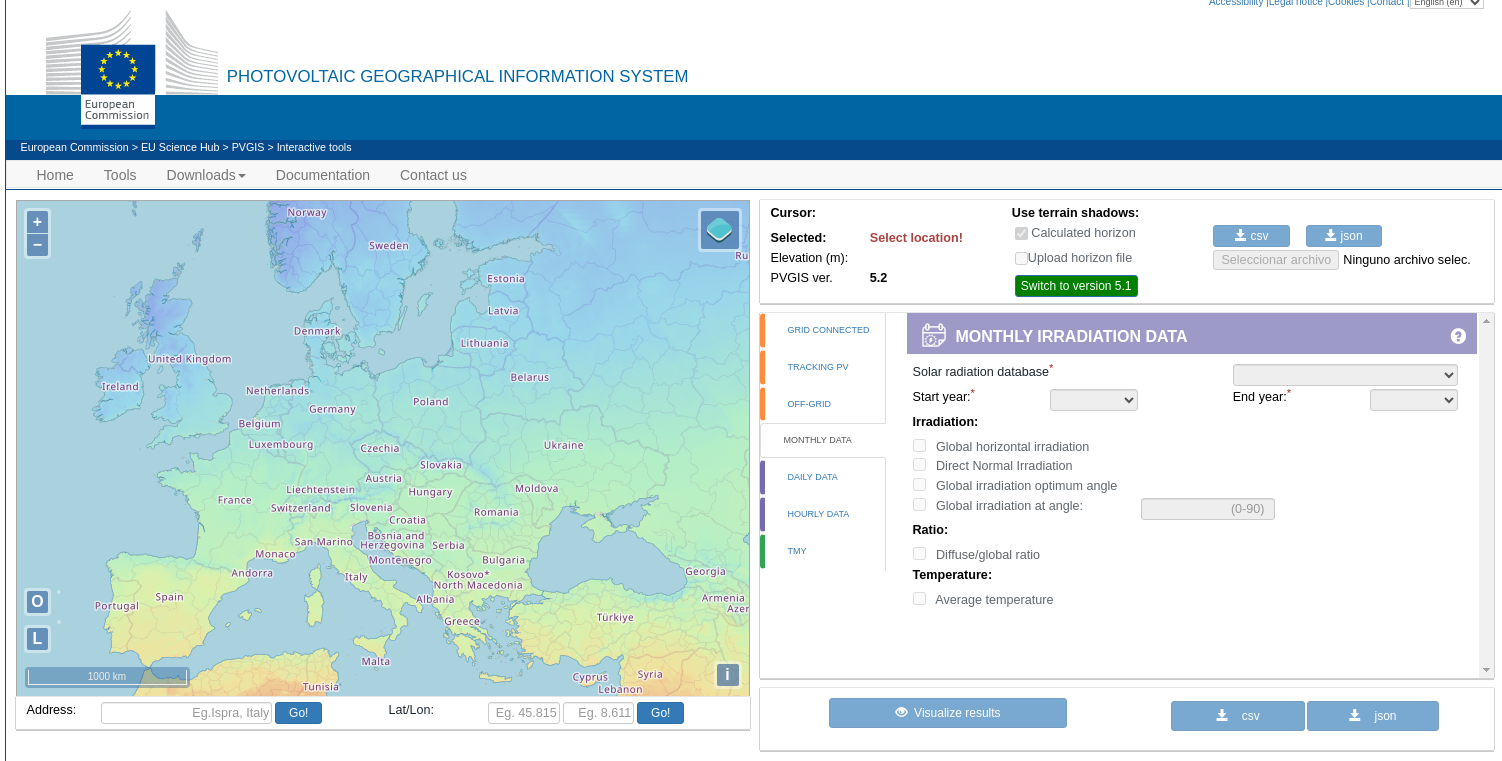
\includegraphics[height=0.35\textwidth]{../figs/pvgis.png}
\end{center}
\end{block}
\end{frame}

\section{Control de calidad}
\label{sec:orgb4a2972}
\begin{frame}[label={sec:orgbf46a1c}]{Introducción}
Las medidas recogidas por estaciones meteorológicas se deben filtrar para eliminar datos erróneos.

Para valores de \alert{irradiación diaria} destacan:

\begin{itemize}
\item Límites Físicos
\item Coherencia espacial
\end{itemize}
\end{frame}


\begin{frame}[label={sec:orge5fdcfa}]{Límites físicos: Irradiación Diaria}
\begin{itemize}
\item La radiación global en el plano horizontal debe ser inferior a la extraterrestre (\(K_{td} \leq 1\))
\end{itemize}
\[
G_d(0) \leq B_{od}(0)
\]

\begin{itemize}
\item El índice de claridad debe ser superior a 0.03
\end{itemize}
\[
K_{td} = \frac{G_d(0)}{B_{od}(0)} \geq 0.03
\]

\begin{itemize}
\item La radiación global en el plano horizontal debe ser inferior a la de un modelo de cielo claro
\end{itemize}
\end{frame}

\begin{frame}[label={sec:org8f9f212}]{Coherencia espacial: planteamiento}
\begin{itemize}
\item Las medidas de una estación se pueden comparar con las recogidas por estaciones cercanas.
\item Esta comprobación debe realizarse con \alert{datos agregados} (diarios) (la variabilidad espacial intradiaria puede ser alta)
\item Esta comprobación debe realizarse con estaciones que tienen \alert{clima y geografía similar}.
\end{itemize}
\end{frame}


\begin{frame}[label={sec:orga1d773c}]{Coherencia espacial: procedimiento}
\begin{itemize}
\item Estimamos la irradiación en el lugar, \(x_0\), con la interpolación espacial de las estaciones cercanas, \(x_i\).
\[
\widehat{G}_d(x_0) = \frac{\sum_{i=1}^N w_i G_{d}(x_i)}{\sum_{i=1}^N w_i} 
\]
Los pesos \(w_i\) son una función inversa de la distancia \(d\) entre las estaciones (IDW).
\[
  w_i = 1/d^2(x_0, x_i)
\]

\item Comparamos la irradiación estimada, \(\widehat{G}_d(x_0)\), con la medida en la estación, \(G_d(x_0)\).
\end{itemize}
\[
\left| \widehat{G}_d(x_0) - G_d(x_0) \right|
\]
\begin{itemize}
\item La diferencia absoluta debe estar por debajo de un límite (p.ej. 50\%)
\end{itemize}
\end{frame}


\begin{frame}[label={sec:org5c31d0a}]{Métricas para diferencias}
\begin{itemize}
\item Mean Bias Difference (MBD), diferencia media (indica si la medida, X,  está por encima o debajo de la referencia, \(R\)):
\end{itemize}
\[
MBE = \overline{\mathbf{D}} = \overline{\mathbf{X}} - \overline{\mathbf{R}} = \frac{1}{n} \sum_{i=1}^n (x_i - r_i)
\]

\begin{itemize}
\item Root Mean Square Difference (RMSD), diferencia cuadrático media:
\end{itemize}
\[
RMSD = \left(\frac{1}{n} \sum_{i=1}^n d_i^2 \right)^{1/2} =  \left( \frac{1}{n} \sum_{i=1}^n (x_i - r_i)^2  \right)^{1/2}
\]

\begin{itemize}
\item Mean Absolute Deviation (MAD):
\end{itemize}

\[
MAD = \frac{1}{n} \sum_{i=1}^n \left|d_i\right| =  \frac{1}{n} \sum_{i=1}^n \left|x_i - r_i\right|
\]
\end{frame}
\end{document}
